\documentclass[border=3pt,tikz]{standalone}
% Shared look for every TikZ figure in these notes.
% Included by each standalone figure file; also keeps the figures consistent
% with the colours used in the PDF and on the website.

\usepackage{tikz}
\usepackage{pgfplots}
\pgfplotsset{compat=1.18}
\usetikzlibrary{arrows.meta, decorations.markings, decorations.pathmorphing,
                patterns, calc, positioning}
\usepackage{amsmath}

% Series colours are the three validated categorical slots also used by the
% interactive widgets, so a path drawn in the printed notes and the same path on
% the website are the same colour. They clear the colour-vision-deficiency and
% contrast checks as a set; every path is direct-labelled as well, so colour is
% never the only thing carrying identity.
\definecolor{duPurple}{HTML}{68246D}
\definecolor{duBlue}{HTML}{2A78D6}
\definecolor{duRed}{HTML}{EB6834}
\definecolor{duGreen}{HTML}{1BAF7A}
\definecolor{duGrey}{HTML}{4D4D4D}

\tikzset{
  % heavier default lines and arrow tips, so diagrams stay clear when zoomed
  every picture/.append style = {line width=0.7pt, >={Stealth[length=3mm]}},
  axisline/.style   = {-{Stealth[length=3.4mm]}, line width=1.0pt, black},
  path1/.style      = {duBlue,   line width=1.6pt},
  path2/.style      = {duRed,    line width=1.6pt},
  path3/.style      = {duGreen,  line width=1.6pt},
  statedot/.style   = {circle, fill=black, inner sep=1.8pt},
  arrowhead/.style  = {decoration={markings,
                        mark=at position #1 with {\arrow{Stealth[length=3.4mm]}}},
                       postaction={decorate}},
  lbl/.style        = {font=\normalsize},
  slbl/.style       = {font=\small, duGrey},
  workfill/.style   = {duPurple, opacity=0.16},
}

% larger labels in plots as well
\pgfplotsset{every axis/.append style={label style={font=\normalsize}, tick label style={font=\small}, line width=0.9pt}}

% Towards equilibrium: a ball settling in a bowl, two blocks reaching one
% temperature, a gas spreading through a box.
\begin{document}
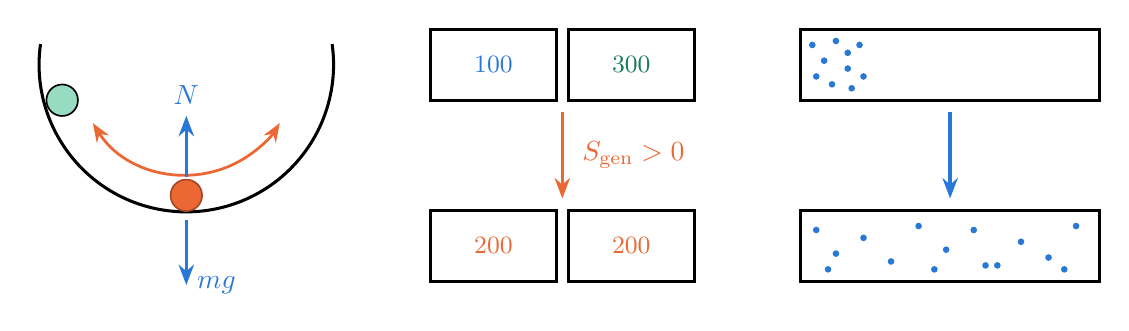
\begin{tikzpicture}[x=1cm,y=1cm,
    flow/.style={-{Stealth[length=2.6mm]}, line width=1.2pt},
    blk/.style={draw=black, line width=1.1pt, minimum width=1.6cm,
                minimum height=0.9cm, inner sep=0, font=\small}]
  % --- ball in a bowl ----------------------------------------------------
  \draw[line width=1.1pt] (0,0.3) ++(172:1.87) arc[start angle=172, end angle=368, radius=1.87];
  \fill[duGreen!45, draw=black, line width=0.6pt] (0,0.3) ++(196:1.64) circle (0.2);
  \fill[duRed, draw=duRed!70!black, line width=0.6pt] (0,-1.36) circle (0.2);
  \draw[{Stealth[length=2.4mm]}-{Stealth[length=2.4mm]}, line width=1.0pt, duRed]
    (0,0.3) ++(212:1.4) arc[start angle=212, end angle=328, radius=1.4];
  \draw[flow, duBlue] (0,-1.13) -- (0,-0.35) node[above, lbl] {$N$};
  \draw[flow, duBlue] (0,-1.67) -- (0,-2.5) node[right, lbl] {$mg$};
  % --- two blocks in contact ---------------------------------------------
  \begin{scope}[shift={(3.9,0)}]
    \node[blk] at (0,0.3)  {\textcolor{duBlue}{$100$}};
    \node[blk] at (1.75,0.3) {\textcolor{duGreen!70!black}{$300$}};
    \node[blk] at (0,-2.0) {\textcolor{duRed}{$200$}};
    \node[blk] at (1.75,-2.0) {\textcolor{duRed}{$200$}};
    \draw[flow, duRed] (0.875,-0.3) -- (0.875,-1.4);
    \node[lbl, duRed, right] at (1.0,-0.85) {$S_\text{gen} > 0$};
  \end{scope}
  % --- gas spreading through a box ---------------------------------------
  \begin{scope}[shift={(9.7,0)}]
    \draw[line width=1.1pt] (-1.9,-0.15) rectangle (1.9,0.75);
    \draw[line width=1.1pt] (-1.9,-2.45) rectangle (1.9,-1.55);
    % before: the gas is all in one corner
    \foreach \x/\y in {-1.75/0.55, -1.6/0.35, -1.45/0.6, -1.3/0.45, -1.15/0.55,
        -1.7/0.15, -1.5/0.05, -1.3/0.25, -1.1/0.15, -1.25/0.0}
      \fill[duBlue] (\x,\y) circle (1.2pt);
    % after: it fills the whole box
    \foreach \x/\y in {-1.7/-1.8, -1.45/-2.1, -1.1/-1.9, -0.75/-2.2, -0.4/-1.75,
        -0.05/-2.05, 0.3/-1.8, 0.6/-2.25, 0.9/-1.95, 1.25/-2.15, 1.6/-1.75,
        -1.55/-2.3, -0.2/-2.3, 0.45/-2.25, 1.45/-2.3}
      \fill[duBlue] (\x,\y) circle (1.2pt);
    \draw[flow, duBlue] (0,-0.3) -- (0,-1.4);
  \end{scope}
\end{tikzpicture}
\end{document}
